\section{Dataset Construction}
\label{sec:dataset}

The dataset is the substrate on which every later claim rests. We describe (i) why we built it from scratch, (ii) the workload we instrumented and the production-realism discipline that governed every change, (iii) the scenario library and fault-injection mechanisms, (iv) the telemetry export pipeline, (v) per-window labeling, and (vi) the humanized Jira corpus.

\subsection{Why a controlled lab, not real production data}

Two structural problems make public datasets insufficient. First, no public corpus jointly contains rich telemetry \emph{and} linked Jira tickets with both pre-incident triggers and post-incident resolutions. Open log datasets carry no ticket-side ground truth; the largest public Jira dataset (TAWOS, 458K real Jira issues across multiple projects~\cite{tawos}) carries no co-collected telemetry. We use TAWOS only as a length/style reference, never as labeled training data.

Second, real production telemetry from cooperating organizations is rarely shareable for legal, privacy, and competitive reasons. Even when shareable, it is rarely \emph{reproducible}: an external reviewer cannot regenerate the data from scratch to check a claim.

A controlled lab solves both. We pay the cost of synthetic-but-realistic data in exchange for full provenance: every test number we report can be traced back to a fault-injection script, a telemetry export, a derived feature pipeline, and a deterministic build step.

\subsection{Workload: Online Boutique with production-realistic instrumentation}

The workload is Google's Online Boutique~\cite{online-boutique}, a ten-service e-commerce microservices demo with services written in Go (frontend, checkoutservice, productcatalogservice, shippingservice), C\#/.NET (cartservice), Node.js (paymentservice, currencyservice), Python (recommendationservice, emailservice, loadgenerator), and Java (adservice). We forked the upstream repository to a branch \texttt{master-yuvraj-fork} and ran five sequential instrumentation phases (M0--M5) over $\sim$3 weeks.

\paragraph{The bias-avoidance discipline.}
Every change we made to the microservices was constrained by a single hard rule: \emph{any field a real production service would not emit must not be added}. Concretely, we rejected scenario IDs in span attributes, fault-type labels in log fields, alert names tied to our scenario taxonomy, and any field listed in our \texttt{triage-task-contract.md} field policy as evaluation-only. The rationale is that our research is operationally meaningful only if the telemetry our models train on resembles the telemetry a real SRE team would have. If we leak scenario labels into the telemetry stream, the resulting numbers describe an unrealistic surrogate task.

This discipline produces a less convenient dataset (debugging label leakage is harder than relying on direct labels) but a defensible one. We have rejected ideas that would have ``helped our model'' specifically because they failed the realism test.

\paragraph{What we added.}
Across three categories of telemetry, the modifications were:

\textbf{Logs (L1--L3).} (L1) A per-RPC structured request log via shared per-language interceptor middleware (Go \texttt{logrus} JSON, .NET \texttt{Microsoft.Extensions.Logging}, Node \texttt{pino}, Python stdlib \texttt{logger}, Java SLF4J). Each interceptor emits one JSON line per RPC carrying \texttt{trace\_id}, \texttt{method}, \texttt{peer\_service}, \texttt{latency\_ms}, \texttt{status\_code}, and \texttt{err\_class}. (L2) Structured error context at dependency boundaries: wherever a service calls Redis, a downstream gRPC service, or an external HTTP API, the failure path logs \texttt{\{dep, op, err\_class, retry\_attempt\}}. (L3) A small business-event layer: \texttt{cart\_size\_changed}, \texttt{order\_placed}, \texttt{payment\_charged}, \texttt{recommendation\_returned\_n\_items}. None of these encode scenario identity.

\textbf{Traces (T1--T5).} (T1) Bringing the three unloved services---cartservice, adservice, shippingservice---to OpenTelemetry parity with the rest of the fleet. Cartservice received \texttt{OpenTelemetry.Instrumentation.AspNetCore}, \texttt{OpenTelemetry.Instrumentation.GrpcNetClient}, and crucially \texttt{OpenTelemetry.Instrumentation.StackExchangeRedis}, the last of which gives per-Redis-operation spans automatically. Adservice received the OpenTelemetry Java agent (drop-in JAR). Shippingservice received the same \texttt{otelgrpc} interceptors as the other Go services. (T2) \texttt{RecordError(err)} and \texttt{SetStatus(Error)} on every error-returning handler. (T3) Manual child spans for dependency calls with semantic-convention attributes (\texttt{db.system}, \texttt{db.operation}, \texttt{net.peer.name}, \texttt{rpc.grpc.status\_code}). (T4) Span events for retries, cache hits/misses, fallbacks. (T5) We \emph{leave} sampling at \texttt{AlwaysSample()}---a known divergence from production (typically 1--10\% head sampling)---and document it explicitly. Dataset density was favored over sampling realism.

\textbf{Metrics (M1--M4).} (M1) An OpenTelemetry \texttt{MeterProvider} with the Prometheus exporter on every service, emitting RED (Rate / Errors / Duration) metrics per RPC handler. (M2) Per-outbound-dependency client metrics labeled by \texttt{peer\_service} and \texttt{operation}. (M3) A small set of business-event counters (\texttt{orders\_placed\_total}, \texttt{payments\_total}, \texttt{cart\_operations\_total})---carefully chosen to never have label values that mirror our scenario taxonomy. (M4) Standard runtime gauges via each language's Prometheus client default (Go GC, .NET GC, Python GC, Node heap, process FDs).

\textbf{The single highest-leverage change} was T1's StackExchange.Redis instrumentation on cartservice. Cart-Redis incidents account for the largest scenario family in our dataset (137 windows in the in-distribution test split), and prior to T1 cartservice emitted zero OpenTelemetry spans. M5 validation pilots confirmed mean \texttt{trace\_error\_count} on cart-Redis active-fault windows rose 3.0$\times$ and nonzero-fraction rose from 50\% to 100\% after the cartservice OTel upgrade.

\subsection{Observability stack}

We deployed Loki for log aggregation, Tempo for distributed traces, Prometheus for metrics, Alertmanager for alert routing, and Grafana Alloy as the OpenTelemetry collector. Every signal carries the four research-injection labels (\texttt{DATASET\_RUN\_ID}, \texttt{SCENARIO\_ID}, \texttt{TRAFFIC\_PROFILE\_ID}, \texttt{JIRA\_MODE}) at the namespace level so windows can be linked back to their generating scenario without polluting application-level telemetry. The full stack runs on a 3-node kind cluster (15.34 GiB host memory budget, $\sim$10--13 GiB sustained for the full workload) for development; the large-scale collection used a Google Cloud Engine \texttt{e2-standard-16} VM.

\subsection{Scenario library}

The dataset covers 27 scenario families spanning the operationally interesting space. Table~\ref{tab:scenario-families} groups them by fault category.

\begin{table}[h]
\centering
\caption{Scenario family taxonomy (27 families).}
\label{tab:scenario-families}
\small
\begin{tabularx}{\linewidth}{l X}
\toprule
Category & Families \\
\midrule
Hard service outage & \texttt{payment-outage}, \texttt{checkout-outage}, \texttt{currency-outage}, \texttt{shipping-outage}, \texttt{recommendation-outage}, \texttt{ad-outage}, \texttt{productcatalog-outage}, \texttt{email-outage} \\
Dependency degradation & \texttt{cart-redis}, \texttt{productcatalog-latency} \\
Pod restart / churn & \texttt{checkout-restart}, \texttt{frontend-restart}, \texttt{single-pod-restart-healthy-replication}, \texttt{flapping-pod}, \texttt{post-deploy-churn} \\
Capacity / traffic pressure & \texttt{frontend-traffic-pressure}, \texttt{scheduled-job-spike}, \texttt{resource-saturation}, \texttt{slow-leak-saturation} \\
Near-misses & \texttt{latency-near-miss-partial-recovery}, \texttt{recovered-in-window}, \texttt{third-party-blip} \\
System / network & \texttt{network-latency}, \texttt{network-packet-loss}, \texttt{network-partition}, \texttt{dns-outage} \\
Baseline & \texttt{baseline-normal} \\
\bottomrule
\end{tabularx}
\end{table}

Fault-injection mechanisms span four primitives: (i) \texttt{SetEnv} (patch deployment environment variables, wait for rollout, restore), (ii) \texttt{ScaleDeployment} (scale to zero, restore replicas), (iii) \texttt{RestartPods} (delete pods matching a selector, wait for replacements), and (iv) \texttt{RecordOnly} (passive observation for baseline windows). For example, \texttt{productcatalog-latency-major} sets \texttt{EXTRA\_LATENCY=750ms} on \texttt{productcatalogservice}; \texttt{cart-redis-degradation-critical} scales \texttt{redis-cart} to zero replicas and restores after the active fault window; \texttt{paymentservice-unavailable-critical} scales \texttt{paymentservice} to zero.

\subsection{Run orchestration and the telemetry export pipeline}

A dataset run is a sequence of scenarios executed against a freshly-deployed cluster, with raw evidence preserved at three layers:

\begin{itemize}
\item \textbf{Layer 1 (raw evidence)} under \texttt{data/runs/<run\_id>/}: \texttt{manifest.json}, \texttt{episodes.jsonl}, \texttt{telemetry\_windows.jsonl}, per-window Loki / Prometheus / Tempo / Kubernetes exports under \texttt{raw/}, \texttt{alerts.jsonl}, and \texttt{jira\_shadow\_issues.jsonl}.
\item \textbf{Layer 2 (per-run derived)} under \texttt{data/derived/<run\_id>/}: \texttt{triage\_examples.jsonl} (one row per window with label and 94 derived features), \texttt{window\_memory\_matchings.jsonl} (ground-truth past-ticket links with \texttt{is\_novel} flag), \texttt{windows.jsonl} (model-ready evidence summaries), and \texttt{issues.jsonl} (this run's shadow Jira contributions to the corpus).
\item \textbf{Layer 3 (global)} under \texttt{data/derived/global/<global\_id>/}: \texttt{global-triage-examples.jsonl} (all windows from all runs, with the split manifest), \texttt{jira-memory-corpus.jsonl} (time-ordered ticket corpus with \texttt{available\_as\_memory\_from} timestamps), \texttt{triage-split-manifest.json} (train/val/test plus leave-one-family-out folds), and pipeline-input schema files.
\end{itemize}

The orchestration scripts (\texttt{collect-dataset-run.ps1}, \texttt{run-scenario.ps1}, \texttt{export-telemetry-window.ps1}, \texttt{validate-dataset-run.ps1}) are PowerShell wrappers around the kubectl/REST APIs of the observability stack. Validation enforces that every record carries \texttt{dataset\_run\_id}, every episode has at least one window, every Jira-shadow issue links to an episode and at least one window, raw exports exist for every window, negative windows are present, severities are in \texttt{\{none, minor, major, critical\}}, and time ranges are non-overlapping where expected.

\subsection{Per-window labeling}

Every telemetry window carries:

\begin{itemize}
\item A \textbf{window type} $\in \{$\texttt{observation\_window}, \texttt{pre\_fault\_baseline}, \texttt{active\_fault}, \texttt{recovery\_window}$\}$.
\item A \textbf{triage label} $\in \{$\texttt{noise}, \texttt{borderline}, \texttt{ticket\_worthy}$\}$ (a senior engineer's judgment about whether to file a Jira ticket).
\item A \textbf{novelty label} $\in \{$true, false$\}$ at evaluation time, derived by checking whether any past memory ticket shares the window's \texttt{scenario\_family} and is time-visible at the window's start.
\item A \textbf{matched\_memory\_issue\_ids} list (potentially empty) of past tickets that are the ``gold'' matches for retrieval evaluation.
\item Ninety-four \textbf{derived numeric features} spanning logs (\texttt{log\_error\_count}, \texttt{log\_warning\_count}, \texttt{log\_total\_count}), traces (\texttt{trace\_error\_count}, \texttt{trace\_error\_rate}, \texttt{trace\_latency\_p50\_ms}, \texttt{trace\_latency\_p95\_ms}, \texttt{trace\_count}, \texttt{trace\_span\_count}), Kubernetes (\texttt{k8s\_restart\_count}, \texttt{k8s\_pod\_unavailable\_count}, \texttt{k8s\_warning\_event\_count}), per-service RPC metrics (\texttt{m05\_rpc\_server\_*}, \texttt{m05\_rpc\_client\_*}, \texttt{m05\_svc\_*}), business events (\texttt{m05\_orders\_placed\_per\_sec}, etc.), plus delta-from-baseline columns for each.
\item A free-text \texttt{triage\_evidence\_text} field summarizing the visible window for downstream text retrievers.
\end{itemize}

\subsection{The humanized Jira memory corpus}

Generating realistic Jira tickets is harder than generating telemetry. We went through two voice profiles.

\textbf{V1: customer-service voice.} Initial humanizer used a friendly, descriptive style averaging $\sim$800 characters per ticket. Useful as a baseline but unrepresentative of how engineers actually write.

\textbf{V2: engineer voice with embedded code blocks.} A redesign anchored to length and content distributions measured directly on TAWOS, producing $\sim$2400-character tickets with a leading \texttt{description\_code} block (the engineer's first paste of the relevant logs), per-step prose interleaving body text with additional code/log/trace fragments (\texttt{body\_code}), and resolution notes that read like postmortem closure comments. 90.2\% of the 347 V2 tickets carry at least one \texttt{description\_code} block. Generation respects a sanitizer that strips PII, secrets, and any field that would leak scenario identity.

\textbf{Distractor pool.} A 110-ticket pool of memory noise: 60 tickets sampled and re-humanized from TAWOS real Jira (PII-stripped, cross-architecture), 25 in-architecture-but-irrelevant tickets (other Online-Boutique-shaped scenarios with no overlap to our 27 families), and 25 cross-architecture tickets (DB, mobile, infrastructure incidents from outside the microservices domain). Used in robustness experiments at memory-noise ratios of $\{0, 10, 25, 50\}\%$.

\subsection{Final dataset statistics}

\begin{table}[h]
\centering
\caption{Locked dataset statistics (global ID: \texttt{2026-05-25-dataset-v5-large-global}).}
\label{tab:dataset-stats}
\small
\begin{tabular}{lr}
\toprule
Item & Count \\
\midrule
Dataset runs & 100 \\
Scenario families & 27 \\
Total telemetry windows & 6{,}720 \\
v2 in-distribution split: train / val / test & 4{,}701 / 1{,}011 / 1{,}008 \\
Test windows with non-empty gold & 331 \\
Test windows truly novel (no gold match) & 677 \\
Jira memory corpus (V2 engineer-voice) & 347 \\
Distractor pool & 110 \\
Derived numeric features per window & 94 \\
Raw evidence size (logs + traces + metrics + k8s) & $\sim$10 GB compressed \\
\bottomrule
\end{tabular}
\end{table}

The split is chronological and family-stratified: the same scenario family appears in train, val, and test, but with different fault-injection runs in each. This is the ``in-distribution'' regime: we measure whether the system can retrieve past tickets from the same family it has seen. A complementary leave-one-family-out evaluation (Section~\ref{sec:g-series}, G8) tests the harder ``orphan family'' regime.

\begin{figure}[h]
\centering
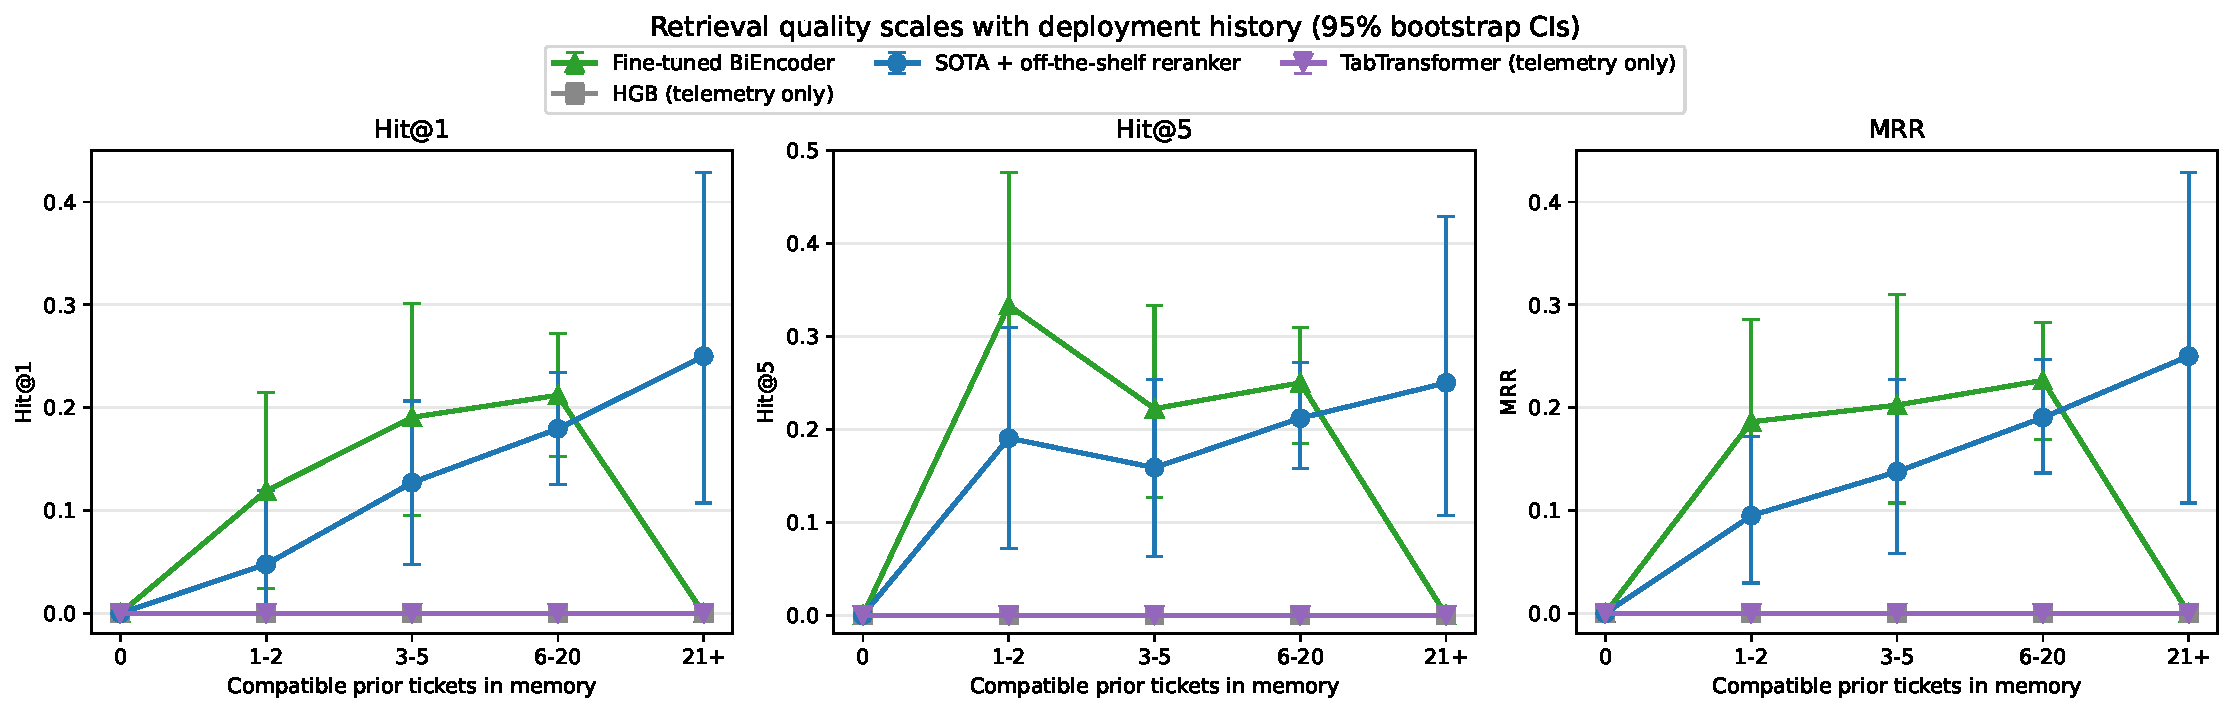
\includegraphics[width=0.92\linewidth]{figures/anchor_combined.pdf}
\caption{Dataset structure: depth-stratified retrieval (Recall@5 vs the number of prior memory tickets sharing the test window's scenario family). The dataset exhibits the operationally-realistic property that retrieval quality scales with deployment history---the underlying motivation for memory-augmented triage and the original Phase A anchor result.}
\label{fig:anchor-depth}
\end{figure}

\subsection{Production-fidelity disclosures}

We document the known divergences from real production telemetry up front:

\begin{enumerate}
\item Trace sampling is 100\% (\texttt{AlwaysSample}); production typically samples 1--10\% head or tail-on-error.
\item Single-cluster, single-region; no cross-AZ failover, no multi-region partitions.
\item No real customer PII; loadgenerator emits synthetic users and synthetic card numbers.
\item Synthetic traffic patterns (no diurnal cycle, no weekly seasonality, no business-hour effect).
\item Single fault per run (real production incidents often have correlated multi-fault cascades).
\item Shadow Jira generated from scenario YAML templates, not engineer-authored.
\item No alert-fatigue baseline (no background false positives from pre-existing alert rules).
\item No GPU-served services (recommendation and ad use CPU sort-by-popularity).
\end{enumerate}

These divergences bound the external validity of our results. The headline claim (memory-augmented retrieval scales with deployment history and detects novelty) is robust across them; latency-magnitude claims and cost claims are not.
